\documentclass[11pt,a4paper]{article}
\usepackage[T1]{fontenc}
\usepackage{lmodern}
\usepackage{textcomp}
\usepackage[margin=2.2cm]{geometry}
\usepackage{xcolor}
\usepackage{listings}
\usepackage{booktabs}
\usepackage{tabularx}
\usepackage{array}
\usepackage{longtable}
\usepackage{tikz}
\usetikzlibrary{positioning,arrows.meta,shapes.geometric}
\usepackage{enumitem}
\usepackage{parskip}
\usepackage[hidelinks]{hyperref}

\setlist{itemsep=2pt,topsep=3pt}
\setlength{\emergencystretch}{2em}
\newcommand{\code}[1]{\texttt{\detokenize{#1}}}
\newcolumntype{L}{>{\raggedright\arraybackslash}X}
\renewcommand{\arraystretch}{1.2}

\definecolor{kw}{RGB}{150,0,110}
\definecolor{cm}{RGB}{90,110,90}
\definecolor{st}{RGB}{170,70,20}
\definecolor{bg}{RGB}{246,247,249}
\lstdefinelanguage{GDScript}{
  morekeywords={func,var,const,if,elif,else,for,in,while,return,match,class_name,extends,signal,static,
    and,or,not,true,false,null,self,super,await,enum,is,as,pass,break,continue},
  sensitive=true,
  morecomment=[l]{\#},
  morestring=[b]",
}
\lstset{
  language=GDScript,
  basicstyle=\ttfamily\small,
  keywordstyle=\color{kw}\bfseries,
  commentstyle=\color{cm}\itshape,
  stringstyle=\color{st},
  backgroundcolor=\color{bg},
  frame=single, rulecolor=\color{black!15},
  framesep=4pt, xleftmargin=6pt, xrightmargin=6pt,
  tabsize=4, breaklines=true, columns=fullflexible, keepspaces=true,
  upquote=true, showstringspaces=false,
  captionpos=b, abovecaptionskip=4pt,
}

\title{\textbf{Parkin' Space: Source Code Guide}\\[4pt]
\large How the game's code is organised and how it works}
\author{Ethan Campomanes \quad BSIT 4C \quad ITSD 85 Lab 5}
\date{November 2026}

\begin{document}
\maketitle

\begin{abstract}
\noindent Parkin' Space is a zero-gravity valet parking game for Android, written in GDScript for the Godot 4 engine. This guide explains the source code for a reader who knows programming but has not opened the project: how the folders and scenes fit together, how a ship flies, how a shift is scored, how progress is saved, how the two-phone online duel stays in sync, and how the code is tested. Short excerpts from the real code are included where they make the explanation clearer. Appendix~A lists every script with a one-line description.
\end{abstract}

\tableofcontents
\newpage

%=====================================================================
\section{Godot in one page}
A few Godot ideas are needed to read the rest of this guide.

\begin{description}[leftmargin=0pt]
\item[Node] The building block of everything: a sprite, a button, a physics body, a timer. Nodes form a tree.
\item[Scene] A saved tree of nodes (a \code{.tscn} file). A level, a ship and a menu screen are each a scene. Scenes can contain other scenes; every level, for example, contains many \code{Ship} scenes at run time.
\item[Script] A GDScript file (\code{.gd}) attached to a node. It adds variables and functions to that node. \code{class_name Ship} gives the script a global type name so other scripts can write \code{var s: Ship}.
\item[Callbacks] Godot calls certain functions automatically: \code{_ready()} once when the node enters the tree, \code{_process(delta)} every drawn frame, \code{_physics_process(delta)} every physics step (60 per second), \code{_draw()} when the node needs repainting, and \code{_unhandled_input(event)} for touches the UI did not use.
\item[Signal] An event a node announces, such as a button's \code{pressed} or a ship's \code{dented}. Other code connects a function to it and is called when it fires. Signals keep nodes from needing to know about each other.
\item[Autoload] A script Godot creates once at start-up and keeps alive across all scenes, reachable by name from anywhere. This project has three: \code{GameState}, \code{Sound} and \code{Net}.
\item[Resource] A saved data object (\code{.tres}), like a ship's specification. Resources hold data; they do not run every frame.
\item[RefCounted] A plain object that is not a node. The project uses these for pure rule classes such as \code{ShiftLedger} and \code{Customer}, which makes them easy to test without a running scene.
\end{description}

%=====================================================================
\section{The project at a glance}
The game has about 7{,}300 lines of game code in 57 scripts, plus 36 test files. Table~\ref{tab:folders} shows where things live.

\begin{table}[h]
\centering
\begin{tabularx}{\textwidth}{@{}lL@{}}
\toprule
\textbf{Folder} & \textbf{What is in it} \\
\midrule
\code{autoload/} & Always-alive services: \code{GameState} (progress, settings, save file) and \code{Sound} (effects and music). \\
\code{scripts/} & \code{Level.gd} (the core of a shift), \code{TutorialLevel.gd} and \code{DuelLevel.gd}, which both extend it. \\
\code{scripts/core/} & Pure data and rules: ship and thruster specs, parking rules, the pay ledger, customers, orphans, valets, the ship-art builder. \\
\code{scripts/actors/} & Things in the lot: \code{Ship}, \code{ParkingSpace}, \code{ExitPad}, \code{ArrivalBay}, \code{Asteroid}, \code{Wreck}, \code{BlackHole}, \code{RadiationZone}, \code{Floodlight}, \code{LotEdge}. \\
\code{scripts/net/} & The online duel: connection (\code{NetSession}), match messages (\code{NetSync}), binary packing (\code{NetProtocol}), the guest's view (\code{GuestMirror}, \code{SnapshotBuffer}) and duel arrivals. \\
\code{scripts/ui/} & Every screen and on-screen control: title, menus, HUD, driving pad, ship picker, pause menu, How to Play guide, tutorial pointer and signs. \\
\code{scripts/fx/} & Full-screen effects: the CCTV video filter and the speed warning glow. \\
\code{scenes/} & The \code{.tscn} files: \code{levels/} (Tutorial, Level01--05, Duel), \code{actors/}, \code{ui/}. \\
\code{resources/ships/} & Ten ship specifications (\code{.tres}) built from the pixel art. \\
\code{art/}, \code{assets/} & Ship art and marker images; audio, fonts, the UI theme. \\
\code{tools/} & Editor-time scripts: build ships from art, make the app icon, check the Android export. \\
\code{tests/} & The headless test runner and 495 automated tests. \\
\bottomrule
\end{tabularx}
\caption{Project folders.}\label{tab:folders}
\end{table}

\subsection{Design rule: rules apart from nodes}
Wherever possible, game rules live in small \code{RefCounted} classes or \code{static} functions that take numbers in and give numbers out. For example, \code{ShiftLedger.dent_cost(speed)} decides what a crash costs, and \code{ParkingRules.is_settled(speed, spin)} decides whether a ship has stopped. The node scripts (\code{Level}, \code{Ship}) gather the inputs, call these rules and show the result. This split is what made 495 tests practical: a rule can be tested in one line without loading a level.

%=====================================================================
\section{Screen flow}
Figure~\ref{fig:flow} shows how the screens connect. Each screen is a scene; moving between them is one call, \code{get_tree().change_scene_to_file(path)}. Every screen also has a \code{back_target()} function that says where Android's back gesture goes.

\begin{figure}[h]
\centering
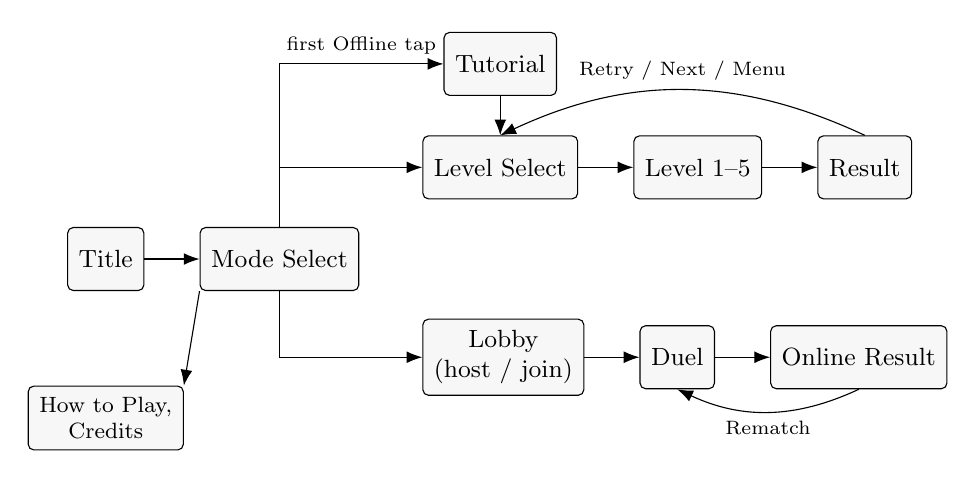
\begin{tikzpicture}[
  box/.style={draw, rounded corners=2pt, align=center, font=\small, minimum height=0.8cm, inner sep=4pt, fill=black!3},
  arr/.style={-{Latex[length=2mm]}},
  node distance=0.5cm and 0.7cm]
\node[box] (title) {Title};
\node[box, right=of title] (mode) {Mode Select};
\node[box, above right=0.35cm and 0.8cm of mode] (level) {Level Select};
\node[box, below right=0.35cm and 0.8cm of mode] (lobby) {Lobby\\(host / join)};
\node[box, above=0.5cm of level] (tut) {Tutorial};
\node[box, right=of level] (lv) {Level 1--5};
\node[box, right=of lv] (res) {Result};
\node[box, right=of lobby] (duel) {Duel};
\node[box, right=of duel] (ores) {Online Result};
\node[box, below=1.2cm of title, font=\footnotesize] (side) {How to Play,\\Credits};
\draw[arr] (title) -- (mode);
\draw[arr] (mode) |- (level);
\draw[arr] (mode) |- (lobby);
\draw[arr] (mode.south west) -- (side.north east);
\draw[arr] (mode.north) |- node[pos=0.75, above, font=\scriptsize]{first Offline tap} (tut.west);
\draw[arr] (tut) -- (level);
\draw[arr] (level) -- (lv);
\draw[arr] (lv) -- (res);
\draw[arr] (res.north) to[bend right=25] node[above, font=\scriptsize]{Retry / Next / Menu} (level.north);
\draw[arr] (lobby) -- (duel);
\draw[arr] (duel) -- (ores);
\draw[arr] (ores.south) to[bend left=25] node[below, font=\scriptsize]{Rematch} (duel.south);
\end{tikzpicture}
\caption{Screens and how the player moves between them.}\label{fig:flow}
\end{figure}

The first time the player taps \emph{Offline}, \code{ModeSelect} sends them straight to the tutorial (it checks \code{GameState.tutorial_seen}); after that, Offline opens Level Select.

%=====================================================================
\section{Saved progress: \texttt{GameState}}
\code{GameState} (\code{autoload/GameState.gd}) remembers everything that must survive between screens and between app launches: the highest unlocked level, the best stars per level, whether the tutorial was seen, and the settings (music, sound effects, difficulty, CCTV strength, duel length, last IP typed).

It writes these to \code{user://save.cfg} using Godot's \code{ConfigFile}, an INI-style text file. On Android, \code{user://} is the app's private storage, so no permission is needed and other apps cannot read it.

\begin{lstlisting}[caption={Clearing a level unlocks the next one and saves at once (\code{GameState.gd}).}]
func complete_level(level: int, stars: int) -> void:
	best_stars[level] = maxi(stars, best_stars.get(level, 0))
	if level == unlocked_level and level < TOTAL_LEVELS:
		unlocked_level = level + 1
	save_progress()
\end{lstlisting}

Saving immediately (rather than when the app closes) means progress survives a force-close. Loading is defensive: each value is read, its type is checked (\code{if level is int}), and it is clamped to a valid range, so a damaged or old save file can never crash the game or unlock a level that does not exist. A setting missing from an older save simply keeps its default.

Level Select asks \code{GameState.is_unlocked(n)} for each button; locked levels are drawn disabled. Difficulty only changes the shift length: Easy 10:00, Normal 5:00, Hard 2:30 (\code{SHIFT_SECONDS}).

%=====================================================================
\section{Ships and flight physics}
\subsection{A ship is data plus a physics body}
Each ship type is a \code{ShipSpec} resource: class (Light, Medium or Heavy), mass, hull outline, centre of mass, and a list of \code{ThrusterSpec}s. Each thruster has a position on the hull, a push direction, a force and the button actions that fire it (\code{thrust_forward}, \code{strafe_left}, \code{rotate_right}, and so on).

The \code{Ship} script extends \code{RigidBody2D}, so Godot's physics engine moves it. Gravity is zero and there is no friction: a ship keeps drifting and spinning until something pushes back. This is the whole challenge of the game.

\subsection{Firing thrusters}
Every physics step, a driven ship asks its \emph{pilot} which buttons are held. A \code{LocalPilot} reads this phone's touch buttons; a \code{NetPilot} reads buttons that arrived over the network (Section~\ref{sec:online}). Each thruster whose action is held pushes the ship \emph{at its own position on the hull}:

\begin{lstlisting}[caption={Each held thruster applies its force at its hull position (\code{Ship._fire_thrusters}).}]
for i in spec.thrusters.size():
	var t := spec.thrusters[i]
	if t.fires_for(held):
		apply_force(global_transform.basis_xform(t.push()),
				global_transform.basis_xform(t.position))
		firing.append(i)
\end{lstlisting}

Because the force is applied off-centre, a thruster that is not lined up with the centre of mass also makes the ship turn. A badly balanced ship therefore twists when it strafes, exactly like a real spacecraft. \code{basis_xform} turns the ship-local vectors into world directions, so ``forward'' always means ``where the nose points''.

\subsection{Stop and Stop Spin}
The \emph{Stop} and \emph{Stop Spin} buttons are brakes. They are done in \code{_integrate_forces}, Godot's hook for changing a body's velocity directly. Stop adds up how much push the ship's thrusters can give against the current drift and slows the ship by at most that much each step; Stop Spin does the same with the rotation thrusters' torque. So a heavy ship with weak retro thrusters genuinely takes longer to stop, and braking never adds sideways force or spin.

\subsection{Collisions and dents}
When a ship touches something, \code{_on_body_entered} works out the impact speed (the difference between the two bodies' velocities just before the hit) and asks the ledger what it costs:

\begin{lstlisting}[caption={The dent price (\code{ShiftLedger.dent_cost}).}]
static func dent_cost(impact_speed: float) -> int:
	if impact_speed <= SAFE_IMPACT_SPEED:   # 120 px/s
		return 0
	return 5 + int((impact_speed - SAFE_IMPACT_SPEED) * 0.25)
\end{lstlisting}

Bumps under 120 pixels per second are free, so careful nudging is allowed. Above that, the cost grows with speed. When two ships collide, exactly one of them reports it (\code{_pays_for_collision_with}) so the player is not charged twice. In a duel, blame follows whoever caused the hit: a ship knocked by a valet carries that valet's mark (\code{last_driver}), so knocking a parked ship into another one still charges the right player.

The speed warning glow (\code{SpeedVignette}) uses the same number: the screen edge is green when slow, yellow at 120~px/s (dents start) and red at 600~px/s. It measures the \emph{fastest point of the hull} (drift plus spin times the hull's reach), because a spinning ship's tip can hit hard even when its centre is slow.

\subsection{Ships from pixel art}
The ship's physics come from its picture. Each ship has two images: the hull art and a \emph{marker} image where single pixels of exact colours mark the engines (red), retro thrusters (blue), side thrusters (green), rotation thrusters (yellow) and centre of mass (magenta). \code{ShipArtBuilder.build} traces the hull outline, groups the marker pixels, works out each thruster's direction from the outline, shares a per-class force budget between them, and computes the moment of inertia from the opaque pixels. The editor tool \code{tools/build_ships.gd} runs this for every ship and writes the \code{.tres} files, so drawing a new ship is enough to add it to the game.

%=====================================================================
\section{Running a shift: \texttt{Level.gd}}
\code{Level.gd} is the largest script (about 1{,}050 lines). Every level scene uses it; the scenes differ only in their layout (walls, spaces, hazards) and in exported settings shown in Table~\ref{tab:levels}.

\subsection{Setup}
When a level loads, \code{_ready()}:
\begin{enumerate}
\item creates one \code{Valet} (the player) and seeds the random number generator;
\item draws this shift's customers (\code{prepare_queue}): a weighted random pick of ships, checked with \code{ParkingRules.fits_lot} so that every drawn ship can actually fit in the lot's spaces at once;
\item picks which customers will later want their ship back, and which will ask for one named space;
\item creates the pay ledger, connects the HUD, driving pad, picker and pause menu by signals;
\item adds the darkness, CCTV filter, ARRIVALS bay marking and red wall outline, then brings in the first ship.
\end{enumerate}

\subsection{The main loop}
Every physics step runs the same fixed order:

\begin{lstlisting}[caption={One physics step of a shift (\code{Level._physics_process}).}]
func _physics_process(delta: float) -> void:
	if _ended:
		return
	for v in valets:
		v.ledger.tick(delta)            # shift clock
	var in_the_way: Array[Node] = _ships.get_children()
	if _asteroids:
		in_the_way.append_array(_asteroids.get_children())
	_update_arrivals(delta, in_the_way) # next customer?
	if _radiation:
		_update_radiation(delta)        # Level 3
	if _black_hole:
		_apply_pull()                   # Level 4
		_fling_from_core()
	_check_parking(delta)               # light up spaces
	_update_customers(delta)            # waits, retrievals
	_update_orphans(delta)              # Level 4
	_refresh()                          # HUD text
\end{lstlisting}

\paragraph{Arrivals.} A new customer arrives once \code{arrival_interval} seconds have passed \emph{and} the ARRIVALS bay has been empty for one second, so a ship never spawns on top of another.

\paragraph{Selecting a ship.} In the lot view, a tap is turned into world coordinates and \code{ships_near_world} finds the ships whose hull is within a thumb-sized radius. One ship is taken directly; several open the \code{ShipPicker} list with numbered badges. Taking a ship switches the camera to follow it and shows the driving pad.

\paragraph{Parking.} Nothing parks by itself. Each step, \code{_check_parking} asks every space whether the driven ship could park there now (\code{ParkingSpace.check}). That needs four things, all in \code{ParkingRules}:
\begin{itemize}
\item the ship's class fits (a Light ship fits any space, a Heavy one only a Heavy space);
\item the space is free;
\item every point of the hull outline is inside the space rectangle;
\item the ship is settled: slower than 10~px/s and spinning slower than 0.2~rad/s.
\end{itemize}
A space that passes turns orange. When the player presses \emph{Done}, \code{press_done} parks the ship in that space; if no space is orange, Done just lets go of the ship.

\paragraph{Being paid.} \code{_on_ship_parked} credits the valet. A customer who will not return is served at once: the 20-credit park fee plus their tip. A customer who will return pays the fee now, and a timer (\code{retrieval_delay}, 20--40 seconds, never so late that the shift could end first) counts down until they ask for the ship back. The ship then glows, and the player must drive it onto the yellow EXIT pad, which hands it over and completes the customer.

\paragraph{Customers and tips.} From Level~2, customers have a tier (\code{Customer.roll}): bronze tips 10 half of the time; silver tips 15, minus 5 per dent; gold tips 40, but only if parked in a gold space, and the tip shrinks by 4 every 5 seconds after 10 seconds of waiting.

\subsection{Winning, losing and stars}
\code{ShiftLedger} keeps the score. The player starts with a base pay of 100 that dents reduce; fees, tips and bonuses go into \code{earned}. The outcome is decided once and never changes:
\begin{itemize}
\item \textbf{Won:} every customer in the queue has been served.
\item \textbf{Fired:} dents took the pay to 0.
\item \textbf{Timeout:} the shift clock reached 0.
\end{itemize}
\code{end_level} then gives stars by total earnings (pay + earned): 1 star for winning, 2 at the level's silver target, 3 at its gold target. A win calls \code{GameState.complete_level}, which unlocks the next level and saves. The result is stored in \code{GameState.last_result} and the Result screen reads it.

\subsection{What changes from level to level}
\begin{table}[h]
\centering\small
\begin{tabularx}{\textwidth}{@{}c c c c L@{}}
\toprule
\textbf{Level} & \textbf{Customers} & \textbf{Silver / gold} & \textbf{Arrives every} & \textbf{New in this level} \\
\midrule
1 & 4 & 150 / 170 & 8 s & Basic flying and parking. \\
2 & 6 & 240 / 280 & 10 s & Customer tiers and tips; 2 customers want their ship back at the EXIT. \\
3 & 7 & 260 / 300 & 10 s & Wrecks (fixed obstacles), drifting asteroids, a radiation zone that dents a ship every 2 s inside it. \\
4 & 7 & 280 / 330 & 10 s & A black hole that pulls moving ships; 2 abandoned ``orphan'' ships to remove. \\
5 & 9 & 360 / 420 & 6 s & Rush hour: 3 customers ask for one named space; parked ships may be moved to make room. \\
\bottomrule
\end{tabularx}
\caption{Level settings, taken from the exported values in each level scene.}\label{tab:levels}
\end{table}

\paragraph{Black hole (Level 4).} \code{BlackHole.pull_at(d)} gives the pull as $1{,}800{,}000/d^2$ px/s$^2$, capped at 80 px/s$^2$, which is weaker than every ship's forward thrust, so the player can always escape. The pull is applied at the centre of mass, so it never spins a ship. Only ships the player has picked up are pulled; a ship parked inside a space is sheltered. Anything that reaches the core is flung out the far side, spinning.

\paragraph{Orphans (Level 4).} Abandoned ships appear in a free space part-way through the shift with a 60-second countdown. Driving one out through the EXIT after the countdown pays a 25 bonus; doing it early costs 15. \code{_allowed_orphan_spaces} only uses spaces whose loss still leaves room for every customer, so an orphan can never make a level impossible.

\subsection{The tutorial}
\code{TutorialLevel} extends \code{Level}, so the tutorial uses the real game rules: the same ship, Done button, orange space and EXIT. It changes only what it must: no shift clock, a ledger that can never fire the player, and ships that arrive only when a step asks for them. It runs 12 steps (``Tap the ship in ARRIVALS'', ``Hold Fwd to go forward'', \dots, ``Now drive it to the EXIT''). Each step has a condition in \code{_step_done()}; every frame, the tutorial advances through all steps whose condition already holds, so a player who does things early simply skips ahead. A \code{TutorialPointer} draws a pulsing ring and arrow at what to tap next, and a \code{TutorialSign} shows the instruction in the lot.

%=====================================================================
\section{The online duel}\label{sec:online}
Two phones on the same Wi-Fi play a timed 1-vs-1 shift in one shared lot. Whoever earns more when the clock runs out wins.

\subsection{Host-authoritative design}
Only the \textbf{host} phone runs the game. It simulates every ship, customer, dent and payment for both players. The \textbf{guest} phone runs no rules at all: it sends its buttons to the host and draws what the host tells it. This means there is only one version of the truth: if both phones ran their own physics, their results could slowly drift apart, and the two players would see different lots. It also means the guest's phone cannot change a score on its own; it can only ask the host.

\begin{figure}[h]
\centering
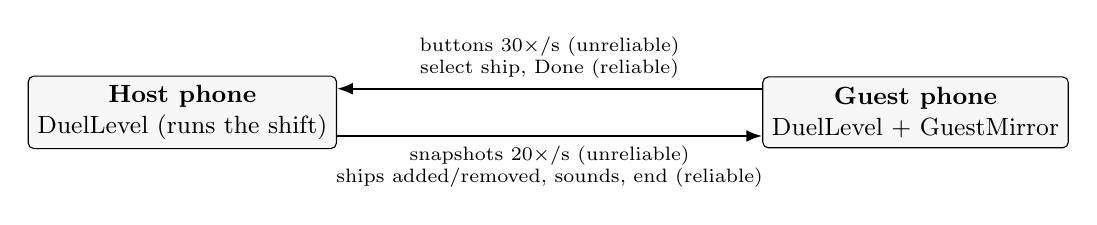
\begin{tikzpicture}[
  box/.style={draw, rounded corners=2pt, align=center, font=\small, minimum width=3.6cm, minimum height=0.9cm, fill=black!3},
  arr/.style={-{Latex[length=2mm]}, thick}]
\node[box] (host) {\textbf{Host phone}\\DuelLevel (runs the shift)};
\node[box, right=5.4cm of host] (guest) {\textbf{Guest phone}\\DuelLevel + GuestMirror};
\draw[arr] ([yshift=3mm]guest.west) -- node[above, font=\scriptsize, align=center]{buttons 30$\times$/s (unreliable)\\select ship, Done (reliable)} ([yshift=3mm]host.east);
\draw[arr] ([yshift=-3mm]host.east) -- node[below, font=\scriptsize, align=center]{snapshots 20$\times$/s (unreliable)\\ships added/removed, sounds, end (reliable)} ([yshift=-3mm]guest.west);
\end{tikzpicture}
\caption{What travels between the two phones during a match.}\label{fig:net}
\end{figure}

On the host, the guest is simply a second \code{Valet} whose ship uses a \code{NetPilot}. Because \code{Level.gd} was written with a list of valets from the start, the duel reuses the whole shift code; \code{DuelLevel} only overrides the parts that differ (two arrival bays, a ledger that only the clock ends, no campaign progress).

\subsection{Connecting: \texttt{NetSession}}
\code{NetSession} (the \code{Net} autoload) wraps Godot's ENet networking on UDP port 24557.
\begin{enumerate}
\item The host calls \code{host()}, which listens for one guest, and shows its Wi-Fi address (\code{pick_lan_ip} skips VPN and virtual adapters and prefers a private 192.168.x.x / 10.x.x.x address).
\item The guest types that address and calls \code{join(ip)}.
\item The guest sends \code{_hello} with its protocol version. If the versions match, the host answers \code{_welcome(minutes)}; if not, \code{_reject()}, and the guest sees ``Your rival has a different version of the game.''
\item If nothing answers within 5 seconds the guest sees ``Cannot reach host. Check that you are on the same Wi-Fi.''
\end{enumerate}

After connecting, each side sends a small \code{_ping} every 0.5 seconds. A \emph{watchdog} counts seconds of silence; after 3 seconds (10 while a scene is loading) the rival is treated as gone, the match ends and the player returns to Mode Select with the message ``Your rival left the match''. This handles Wi-Fi drops and a phone that was simply closed, not only a clean disconnect.

\subsection{Match messages: \texttt{NetSync}}
\code{NetSync} is a node inside the duel scene holding every match message as a Godot RPC (remote procedure call). Every message received is checked: it must come from the connected rival, and requests are only accepted on the host. Table~\ref{tab:msgs} lists them.

\begin{table}[h]
\centering\small
\begin{tabularx}{\textwidth}{@{}l l l L@{}}
\toprule
\textbf{Message} & \textbf{Direction} & \textbf{Delivery} & \textbf{Purpose} \\
\midrule
\code{match_start} & host $\to$ guest & reliable & Random seed, match length, ships already in the lot. Repeated every 0.5 s until the guest answers. \\
\code{loaded} & guest $\to$ host & reliable & The guest's lot is ready; the host starts the 3-2-1 countdown. \\
\code{go} & host $\to$ guest & reliable & Countdown starts on both phones. \\
\code{input} & guest $\to$ host & unreliable, ordered & The guest's held buttons as bits, 30 times a second. \\
\code{select}, \code{done} & guest $\to$ host & reliable & The guest tapped a ship, or pressed Done. The host decides if it is allowed. \\
\code{snapshot} & host $\to$ guest & unreliable & Every ship's position and state, 20 times a second. \\
\code{ship_added}, \code{ship_removed} & host $\to$ guest & reliable & A customer arrived or was handed back. \\
\code{event} & host $\to$ guest & reliable & A sound to play (park, dent, fee). \\
\code{match_end} & host $\to$ guest & reliable & Final scores. \\
\bottomrule
\end{tabularx}
\caption{Duel messages (\code{scripts/net/NetSync.gd}).}\label{tab:msgs}
\end{table}

Button bits and snapshots are sent \emph{unreliable}: if one packet is lost, the next one, 33--50 ms later, replaces it anyway, and resending old positions would only add lag. Everything that happens once (a ship arriving, Done pressed, the final score) is sent \emph{reliable}, so it is never lost.

\subsection{Snapshots in binary}
A snapshot is packed by hand into bytes (\code{NetProtocol.pack_snapshot}) instead of being sent as a Godot dictionary, which keeps each packet small:

\begin{table}[h]
\centering\small
\begin{tabular}{@{}l l l@{}}
\toprule
\textbf{Part} & \textbf{Fields} & \textbf{Bytes} \\
\midrule
Header & tick (u32), time left (float), two scores (2 $\times$ i32) & 16 \\
Lit spaces & count (u8), then which valet each space glows for (i8 each) & 1 + spaces \\
Ships & count (u16), then per ship: & 2 \\
 & \quad id (u16), x, y, rotation (3 $\times$ float) & 14 \\
 & \quad flags (u8: driver, parked, glowing), thrusters firing (u16 bitmask) & 3 \\
\bottomrule
\end{tabular}
\caption{Snapshot layout: 17 bytes per ship.}\label{tab:snap}
\end{table}

A lot with 10 ships and 8 spaces gives about 200 bytes per snapshot, or roughly 4 KB/s at 20 snapshots per second. The unpacker rejects short packets and any packet that claims more than 512 ships, so a malformed packet cannot crash the guest or make it allocate memory without limit.

\subsection{Smooth motion on the guest}
Snapshots arrive 20 times a second, but the screen draws 60 times a second, and packets do not arrive at perfectly even times. \code{SnapshotBuffer} solves this by drawing the lot 0.1 seconds in the past and \emph{interpolating} between the two snapshots on either side of that moment:

\begin{lstlisting}[caption={Blending two snapshots for the moment being drawn (\code{SnapshotBuffer.sample}).}]
var w := (t - _times[i - 1]) / span     # 0..1 between the two
for ship: Dictionary in out.ships:
	if old_by_id.has(ship.id):
		var o: Dictionary = old_by_id[ship.id]
		ship.pos = (o.pos as Vector2).lerp(ship.pos, w)
		ship.rot = lerp_angle(float(o.rot), float(ship.rot), w)
\end{lstlisting}

\code{lerp_angle} takes the short way round, so a ship turning past 180\textdegree{} does not spin the wrong way for one frame. The guest's ships are \emph{frozen} bodies with collisions turned off (built in \code{GuestMirror}); they are only moved to the positions the host sends, and they never collide on the guest.

\subsection{Fair arrivals}
Each player has their own arrival bay. \code{BaySlots} builds a seeded list in which slot $N$ brings a ship of the \emph{same class} and a customer of the \emph{same tier} to both bays, so neither player gets an easier queue. \code{DuelArrivals} keeps a timer per bay and lets a bay that has fallen behind catch up.

%=====================================================================
\section{Presentation: screens, sound and look}
\begin{description}[leftmargin=0pt]
\item[Driving pad] \code{ShipControls} uses Godot's \code{TouchScreenButton}, each mapped to an Input Map action. Multi-touch (thrust and rotate at the same time) works with no extra code, and the same actions are bound to keyboard keys for testing on a computer.
\item[HUD] Goal line, shift clock, pay, customers served, short hints, and a status line such as ``Waiting for customers to return -- next in 0:12'' when everything is parked.
\item[Dark lots] Every lot is pitch black; \code{Floodlight} lamps (some flickering) and each ship's own headlight and glow are the only light. Markings the player must read (spaces, coins, EXIT) use an unlit material so they always show.
\item[CCTV filter] A shader (\code{CctvFilter}) makes the lot look like low-bitrate security camera video, with a ``REC CAM 03'' label and a ticking timestamp. Four strengths, chosen in the pause menu and saved.
\item[Wall warning] \code{LotEdge} draws a red outline inside the walls that brightens as the driven ship's nearest hull point comes within 80 px of a wall.
\item[Sound] The \code{Sound} autoload plays effects from a pool of 8 players (the oldest is reused when all are busy), a looping thruster sound for the driven ship, a menu track, and random level tracks that never repeat back to back. Music and effects have separate buses, so each can be muted.
\item[Neon theme] Every button uses \code{HexStyle}, a custom \code{StyleBox} that draws a glowing hexagon. The driving pad uses the same drawing through \code{HexFace}.
\item[How to Play] \code{Guide} builds its pages from code. Its icons (\code{GuideIcon}) are drawn with the game's own colours and constants, and the ship pages list whatever ships are in \code{resources/ships}, so the guide cannot fall out of date with the game.
\end{description}

%=====================================================================
\section{Testing}
The project has its own small test runner (\code{tests/run_tests.gd}), because it needs nothing beyond Godot itself. It loads every \code{tests/test_*.gd} file, runs each function whose name starts with \code{test_}, and reports passes and failures. A custom \code{Logger} also catches any engine or script error during a test, so a test that crashes half-way is counted as failed, not silently skipped.

The suite runs headless (no window) from the command line:
\begin{lstlisting}[language={}]
godot --headless --path . res://tests/TestRunner.tscn
\end{lstlisting}

\begin{table}[h]
\centering\small
\begin{tabularx}{\textwidth}{@{}lL@{}}
\toprule
\textbf{Kind of test} & \textbf{Examples} \\
\midrule
Pure rules & Dent prices, star thresholds, the gold tip shrinking over time, ``a Heavy ship does not fit a Light space'', \code{fits_lot}, orphan timing. \\
Physics & A ship held on \emph{Fwd} moves the way its nose points; an off-centre thruster spins the ship; weak retro thrusters brake more slowly; the black hole's pull is capped at 80~px/s$^2$. \\
Level behaviour & A level is loaded into the test tree, a ship is placed in a space and Done is pressed; the test checks the pay, the served count and the unlock. \\
Save file & Progress survives saving and reloading; a damaged save file falls back to defaults. \\
Networking & Snapshot packing round-trips exactly; truncated or oversized packets are rejected; a real host and guest connect over \emph{loopback} on one computer and play a match. \\
UI & Every screen's back target; the tutorial advances through all 12 steps; the guide lists every ship. \\
\bottomrule
\end{tabularx}
\caption{What the 495 tests in 36 files cover.}
\end{table}

Tests were written before the code they test (test-driven development): first a failing test that states the wanted behaviour, then the code that makes it pass. All tests were run before every merge into the \code{main} branch, and every build was also installed and played on a Huawei LYA-L29 phone (Android 10).

%=====================================================================
\section{How to build and run}
\begin{itemize}
\item \textbf{Open:} install Godot 4 and open \code{project.godot}. Press F5 to play on the computer (keyboard: W/S/A/D to thrust and strafe, Q/E to rotate, Space to stop, R to stop spinning).
\item \textbf{Test:} run the command in the previous section; it prints \code{ALL TESTS PASSED} at the end.
\item \textbf{Android APK:} \emph{Project $\to$ Export $\to$ Android}, using the preset in \code{export_presets.cfg}. The Android build templates and a debug keystore are required. The keystore and the \code{export/} folder are never committed.
\item \textbf{Online play:} both phones on the same Wi-Fi; one taps \emph{Host} and reads out its address, the other taps \emph{Join} and types it.
\end{itemize}

%=====================================================================
\appendix
\section{Every script}
\small
\begin{longtable}{@{}p{4.3cm}p{11.2cm}@{}}
\toprule
\textbf{Script} & \textbf{What it does} \\
\midrule
\endhead
\multicolumn{2}{@{}l}{\textit{Autoloads}} \\
\code{GameState} & Level progress, best stars, settings, the save file, the last result. \\
\code{Sound} & Effect pool, thruster loop, menu and level music, mute buses. \\
\code{NetSession} (\code{Net}) & LAN connection: host, join, version handshake, keep-alive, silence watchdog, rematch and leave. \\
\midrule
\multicolumn{2}{@{}l}{\textit{Levels}} \\
\code{Level} & One shift: arrivals, ship selection, parking, customers, pay, hazards, end of level, pause. \\
\code{TutorialLevel} & 12-step guided lot on the real rules; no clock, cannot be failed. \\
\code{DuelLevel} & Online duel: roles, countdown, two bays, snapshots to the guest, scores. \\
\midrule
\multicolumn{2}{@{}l}{\textit{Core rules and data}} \\
\code{ShipSpec}, \code{ThrusterSpec} & Ship type data; one thruster's position, push and actions. \\
\code{ShipArtBuilder} & Pixel art and markers to outline, centre of mass, thrusters and inertia. \\
\code{SpriteOutline} & Traces a sprite's opaque pixels into a collision outline. \\
\code{ParkingRules} & Class fit, whole-lot fit, hull inside space, settled. \\
\code{ParkTracker} & Reports once when a condition has held for a set time. \\
\code{ShiftLedger} & Pay, fees, tips, bonuses, timer, outcome, dent cost, stars. \\
\code{Customer} & Tier, tip, waiting time, retrieval and space requests. \\
\code{Orphan} & Abandoned ship's countdown, bonus and early fine. \\
\code{Valet} & One player: ship driven, ledger, pilot, local or remote. \\
\code{ShipPilot}, \code{LocalPilot}, \code{NetPilot} & Where a ship reads its buttons: nobody, this phone, or bits from the network. \\
\code{Lighting} & Shared light textures and the unlit material. \\
\code{Upright} & Keeps world text level on screen whatever the camera's turn. \\
\midrule
\multicolumn{2}{@{}l}{\textit{Actors}} \\
\code{Ship} & Physics ship: thrusters, brakes, lights, badge, dents, collision blame. \\
\code{ParkingSpace} & A space: class, label, gold, occupant, orange when ready, request pin. \\
\code{ExitPad} & The EXIT where ships are handed back. \\
\code{ArrivalBay} & ARRIVALS marking; clear check; pulses while a ship waits; blocks rocks. \\
\code{Asteroid}, \code{Wreck} & Drifting rock; fixed dead ship. \\
\code{BlackHole} & Pull strength, direction and fling. \\
\code{RadiationZone} & Glowing zone that dents ships staying inside. \\
\code{Floodlight} & Lamp with optional flicker; seeded colour in a duel. \\
\code{LotEdge} & Red wall outline that glows as the ship nears a wall. \\
\midrule
\multicolumn{2}{@{}l}{\textit{Online}} \\
\code{NetSync} & All match RPCs, checked against the rival. \\
\code{NetProtocol} & Binary pack/unpack of snapshots and ship lists. \\
\code{SnapshotBuffer} & Guest-side 0.1 s delay and interpolation. \\
\code{GuestMirror} & Guest's view: builds mirror ships, applies snapshots, sends input. \\
\code{BaySlots}, \code{DuelArrivals} & Fair seeded arrival list and per-bay timers. \\
\midrule
\multicolumn{2}{@{}l}{\textit{Screens and UI}} \\
\code{Title}, \code{ModeSelect}, \code{LevelSelect} & Opening screens; tutorial on first Offline tap; level grid and difficulty. \\
\code{Lobby}, \code{OnlineResult} & Host/join and match length; win/lose/draw, rematch, leave. \\
\code{Result} & Outcome, stars, earnings; Retry, Next, Menu. \\
\code{HUD} & Goal, clock, pay, served, hints, status line. \\
\code{ShipControls} & On-screen driving pad and Done. \\
\code{ShipPicker} & List of nearby ships with numbered badges. \\
\code{PauseMenu} & Resume, Restart, sound, CCTV, How to Play, Quit or Leave match. \\
\code{Guide}, \code{GuideIcon} & How to Play pages and their drawn icons. \\
\code{TutorialPointer}, \code{TutorialSign}, \code{TutorialComplete} & Tutorial ring and arrow, instruction sign, end panel. \\
\code{HexStyle}, \code{HexFace} & Neon hexagon buttons. \\
\code{Credits} & Art, sound and music credits and licences. \\
\midrule
\multicolumn{2}{@{}l}{\textit{Effects}} \\
\code{CctvFilter} & Security-camera video shader and overlay. \\
\code{SpeedVignette} & Green/yellow/red screen-edge speed warning. \\
\midrule
\multicolumn{2}{@{}l}{\textit{Tools (editor only)}} \\
\code{build_ships} & Rebuilds every ship \code{.tres} from its art. \\
\code{make_app_icon} & Renders the app icon. \\
\code{check_export_pack} & Checks the Android export contains what it should. \\
\bottomrule
\end{longtable}

\end{document}
